%%%%lezione 25 marzo%%%%


\subsection{Test per la verifica di ipotesi}
Lezione del 25/03, ultima modifica 20/05, Andrea Gadotti
\\ \\

La procedura di test per la verifica di ipotesi che descriveremo a breve cerca di fornire una soluzione ai seguenti problemi:
\begin{enumerate}
\item Determinare quanto un'ipotesi è realistica, verosimile, compatibile con l'informazione empirica a disposizione.
\item Trovare un ragionamento oggettivo (matematico) per inferire dall'informazione disponibile (ovvero il contenuto di un campione) circa la veridicità dell'ipotesi formulata.
\item Misurare in qualche modo questa ''vicinanza'' tra ipotesi e realtà.
\end{enumerate}
Useremo statistiche pivot in ambito parametrico: la distribuzione da cui proviene il campione casuale $(X_1,...,X_n)$ è nota a meno di uno o più parametri.\\
Di seguito si può vedere una descrizione generale della situazione che si riproporrà per tutta questa sezione:\\
\\
$X \sim F_X(\underline{x},\theta)$, $\theta \in \Theta$, $(X_1,...,X_n)$ iid. Le nostre due ipotesi saranno della forma:
$$\bigg \{
\begin{array}{rl}
H_0: & \theta \in \Theta_0 \\
H_1: & \theta \in \Theta_1 \\
\end{array}
$$
con $\Theta_0 \cup \Theta_1 = \Theta$.\\
\\
Chiameremo $H_0$ \textit{ipotesi nulla} e $H_1$ \textit{ipotesi alternativa}. Di solito $H_0$ rappresenta la conoscenza pregressa, la supposizione vera fino a prova contraria. Al contrario, $H_1$ è l'ipotesi di lavoro, quella su cui ripieghiamo nel momento in cui il nostro test risulta in contraddizione con $H_0$.\\
Il test si riduce a una \textit{regola di decisione} in merito a $H_0$ e $H_1$ sulla base del campione casuale $(X_1,...,X_n)$ da $X \sim F_X (x;\theta)$. Dividiamo lo spazio dei campioni in due regioni disgiunte: $C$ (regione critica del test) e $C^c$. La decisione può chiaramente essere corretta, ma anche errata, poiché il campione costituisce un'informazione non completa. Risulta quindi necessario formulare delle \textit{conclusioni in probabilità}, ovvero associare alla nostra conclusione la probabilità che questa sia corretta, cercando ovviamente di massimizzarla.\\
Possiamo riassumere le varie possibilità nella tabella e nel disegno sottostanti:
\\
\\
\begin{center}
\begin{tabular}{c|c|c}
 & $H_0$ è vera & $H_0$ è falsa \\ 
\hline 
Rifiuto $H_0$ & errore di I specie & nessun errore \\ 
\hline 
Non rifiuto $H_0$ & nessun errore & errore di II specie \\ 
\end{tabular} 
\end{center}

\begin{center}
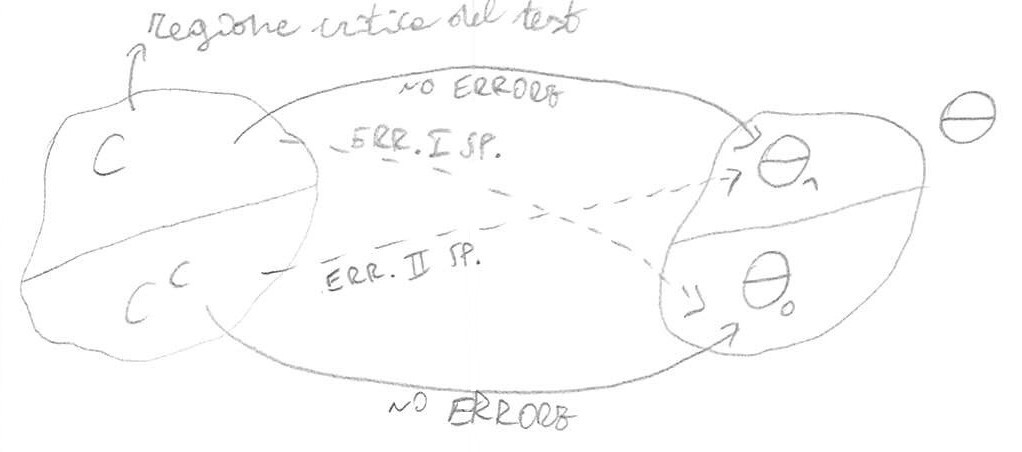
\includegraphics [width=12cm] {immagini/grafico_1.jpg}
\end{center}

\noindent \textbf{Esempio} Lancio di una moneta onesta. Consideriamo il campione casuale $(X_1,...,X_n)$ e il numero di teste $S_n = \sum_{i=1}^n X_i$. Vorremmo stimare la probabilità che esca testa con la media campionaria $\overline{X}_n$. In questo caso potremmo avere:
\\
$$\bigg \{
\begin{array}{rl}
H_0: & p=1/2 \\
H_1: & p \neq 1/2 \\
\end{array}
$$
\\
La regola di decisione consiste quindi nel rifiutare $H_0$ se $(X_1,...,X_n) \in C$ e invece rifiutare $H_0$ se $(X_1,...,X_n) \in C^c$. Ci piacerebbe trovare una regola di decisione che permetta di minimizzare la probabilità di commettere errori di I o II tipo. Purtroppo questo non è possibile, per la natura stessa della relazione che corre tra gli errori di I e II tipo. Di seguito un esempio che ci dà un'idea del perché:\\

\noindent \textbf{Esempio} Consideriamo un campione casuale $(X_1,...,X_n)$ da $N(\mu,\sigma^2)$ con $\sigma^2$ noto. Supponiamo che le nostre due ipotesi siano:
\\
$$\bigg \{
\begin{array}{lcr}
H_0: & \mu=\mu_0 & \text{ovvero } N(\mu=\mu_0,\sigma^2) \\
H_1: & \mu=\mu_1 & \text{ovvero } N(\mu=\mu_1,\sigma^2) \\
\end{array}
$$
con $\mu_1 > \mu_0$.\\
\\
\begin{center}
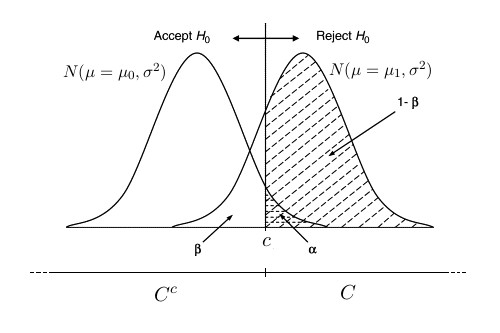
\includegraphics [width=12cm] {immagini/grafico_2.jpg}
\end{center}

Consideriamo $\alpha:= P(\text{rifiutare } H_0 \mid H_0 \text{ vera}) = P(\text{il nostro campione appartiene a C} \mid H_0 \text{ vera}) = P(\text{il nostro campione è } \geq c \mid \text{la distribuzione corretta è quella di sinistra}) = P(\text{commettere un errore di I tipo})$ e $\beta:= P(\text{non rifiutare } H_0 \mid H_0 \text{ falsa}) = P(\text{il nostro campione appartiene a } C^c \mid H_0 \text{ falsa}) = P(\text{il nostro campione è } \leq c \mid \text{la distribuzione corretta è quella di destra}) = P(\text{commettere un errore di II tipo})$. 
(Nota: $\alpha$ è detto \emph{livello di significatività del test})\\
È evidente che non è possibile annullare contemporaneamente sia $\alpha$ che $\beta$.\\
La procedura si divide quindi in due passi: il primo consiste nel \textbf{fissare} $\alpha$, il secondo nell'individuare la regola di decisione che minimizza $\beta$, in modo da trovare un test \textit{ottimo}.\\
\\
\\